% Figure Q4, generated by experiments/q4_local_rate.py.
\begin{figure}[t]
  \centering
  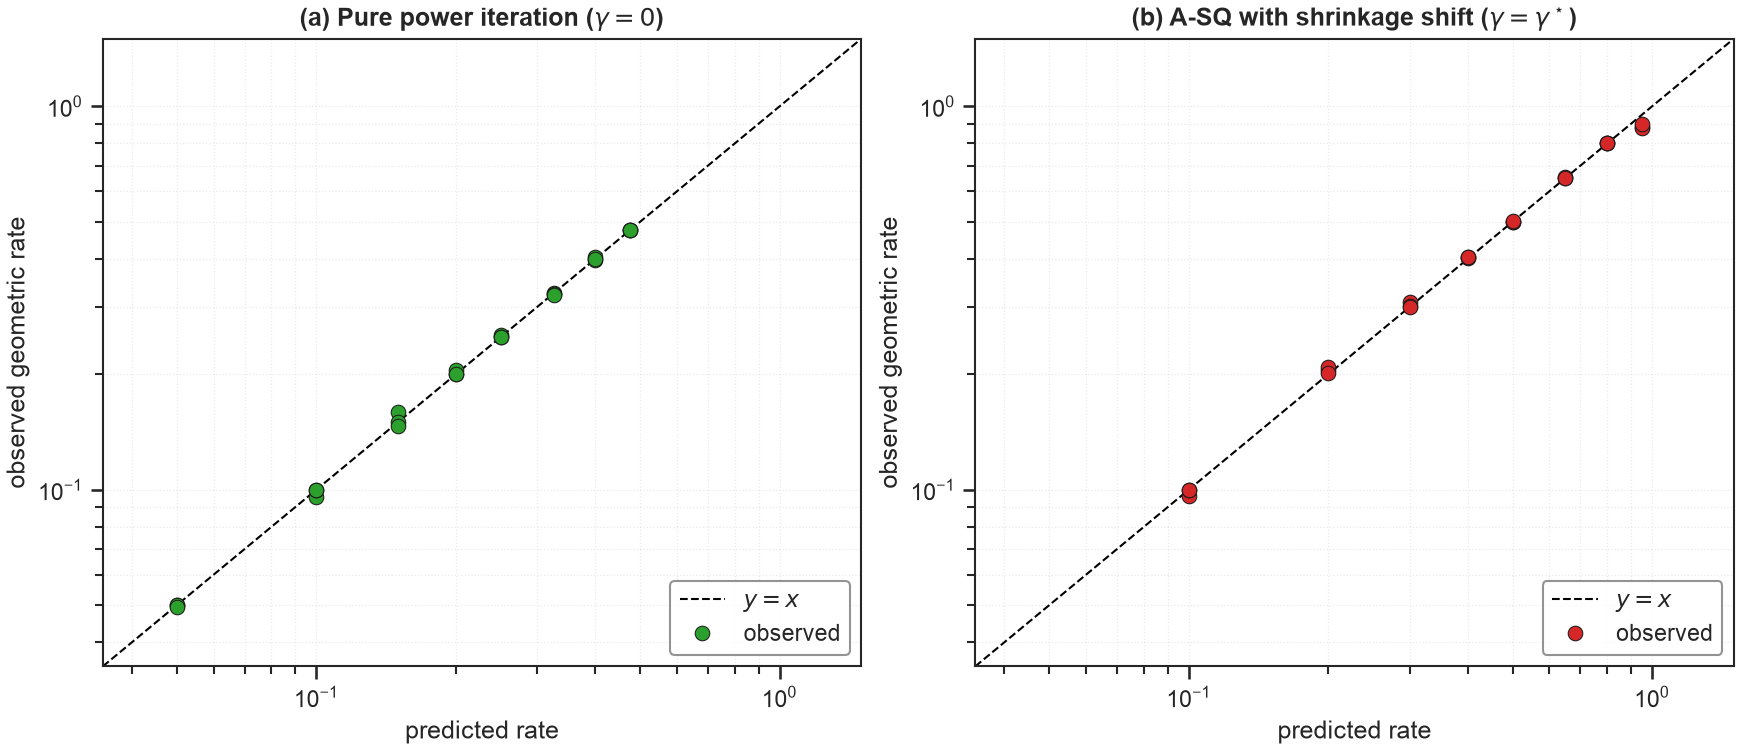
\includegraphics[width=\linewidth]{../shared/figures/generated/q4_local_rate.png}
  \caption{\textbf{Q4, local-rate prediction versus observation: two branches.} Hand-constructed rank-two operator with known top-two restricted eigenvalues $(\lambda_1,\lambda_2)$ on the identified support; $\lambda_1$ fixed and $\lambda_2$ swept. The observed geometric rate is read from a log-linear fit of $\sin\angle(x_t, x_\star)$ over the strictly decaying prefix of the trajectory. \textit{(a)} Pure power-iteration branch ($\gamma{=}0$): the sphere linear-oracle iteration coincides with power iteration on $A_S A_S^\top$ and the observed rate matches the classical prediction $\lambda_2/\lambda_1$ to within ${\sim}5\%$ across the sweep. \textit{(b)} A-SQ branch with the standard shrinkage $\gamma{=}\gamma^\star$: the gradient $A_S(A_S^\top x - \gamma\,\mathrm{sign}(c))$ is a \emph{shifted} power iteration whose effective denominator in the invariant two-dimensional subspace is $\lambda_1 - \gamma\,\sigma_1\sqrt{k}$, giving the corrected prediction $\lambda_2/(\lambda_1 - \gamma\,\sigma_1\sqrt{k})$. Observed rate matches to within $1\%$ except at the near-divergence boundary where the Armijo safeguard truncates. Both panels share the $y{=}x$ reference. Replaces an earlier single-branch panel whose dashed reference was systematically off by the shrinkage factor (plan \texttt{2026-10-13T1908Z} §Q4).}
  \label{fig:q4-local-rate}
\end{figure}
